\documentclass[11pt]{article}
\usepackage{neurips_2023}
\usepackage{colortbl}   % rowcolor — loaded after xcolor from neurips_2023.sty
\usepackage{float}
\usepackage[capitalize]{cleveref}

\graphicspath{{../figures/}{../results/}}

\title{Peptide and Protein Sequencing by Multinomial Diffusion Model\\
\large Checkpoint 2 Report --- CSE 676 Deep Learning, Spring 2026}

\author{%
  Vaishak Girish Kumar\quad Akshay Mohan Revankar\quad Sanika Vilas Nanjan \\
  \texttt{\{vaishakg, arevanka, snajan\}@buffalo.edu} \\
  CSE 676 Deep Learning --- University at Buffalo
}

\begin{document}

\maketitle

\begin{abstract}
We present a multinomial diffusion model for \emph{de novo} peptide sequencing from
tandem mass spectrometry (MS/MS) data. Starting from Checkpoint 1 LSTM/GRU baselines
(31.51\%~/ 44.30\% amino acid recall), Checkpoint 2 introduces four contributions:
(1)~a \textbf{TransformerDenoiser} that performs categorical diffusion over 23 amino
acid tokens conditioned on spectrum context; (2)~an \textbf{entropy-adaptive mass gate}
(Novel~\#1) that enforces precursor mass constraints with per-position tolerance scaled
by denoising entropy; (3)~\textbf{spectral noise augmentation} (Novel~\#4) to improve
generalisation to noisy wastewater spectra; and (4)~an \textbf{ESM-2 pseudo-perplexity}
scorer and \textbf{multi-model ensemble} for post-hoc candidate reranking, plus a
\textbf{target-decoy FDR pipeline} applied to unlabelled wastewater mzML files.
The diffusion model achieves $70.77 \pm 1.52\%$ AA recall across three random seeds,
approaching the InstaNovo reference (72.9\%) while surpassing both baselines by a
large margin.
\end{abstract}

% ─────────────────────────────────────────────────────────────────────────────
\section{Introduction}
% ─────────────────────────────────────────────────────────────────────────────

\emph{De novo} peptide sequencing determines a peptide's amino acid sequence
directly from its MS/MS fragmentation pattern, without a reference proteome.
This is essential for complex metaproteomic samples --- such as wastewater --- where
many organisms are unsequenced and database search is inapplicable.

Current state-of-the-art tools (DeepNovo, Casanovo, InstaNovo) use transformer or LSTM
architectures and treat sequencing as supervised autoregressive generation. While
effective on well-characterised proteomes, they lack physical grounding: they do not
enforce that predicted masses match the observed precursor ion.

We frame \emph{de novo} sequencing as \textbf{discrete denoising diffusion}: iteratively
recovering a clean amino acid token sequence from corrupted noise, conditioned on the
spectrum. Precursor mass constraints are incorporated at every reverse step via a novel
entropy-adaptive gate, providing physically valid predictions. Checkpoint~2 delivers the
full system, benchmarked against both our CP1 baselines and the InstaNovo reference.

% ─────────────────────────────────────────────────────────────────────────────
\section{Methods}
% ─────────────────────────────────────────────────────────────────────────────

\subsection{Diffusion Model Architecture (V-1)}

\paragraph{Encoder.}
Reused from CP1 unchanged: a three-layer MLP
($20{,}000 \to 1{,}024 \to 512 \to 256$) with ReLU activations and Dropout(0.3),
compressing the 20,000-dim binned spectrum into a 256-dim context vector~$\mathbf{s}$.

\paragraph{TransformerDenoiser.}
The denoiser predicts clean $x_0$ directly from noisy input $x_t$, timestep $t$,
and context $\mathbf{s}$:
\begin{itemize}[nosep]
  \item \textbf{Token embedding:} \texttt{nn.Embedding(23, 256)} + learned positional embedding.
  \item \textbf{Timestep embedding:} sinusoidal $\to$ Linear $\to$ 256-dim, added to all positions.
  \item \textbf{Decoder stack:} $4\times$ \texttt{TransformerDecoderLayer}
    ($d_\text{model}=256$, $n_\text{head}=8$, $d_\text{ff}=512$, \texttt{norm\_first=True}),
    cross-attending to $\mathbf{s}$ unsqueezed to $(B\times1\times256)$.
  \item \textbf{Output:} Linear($256\to23$) $\to$ logits $(B, 32, 23)$.
\end{itemize}

\paragraph{Forward process.}
We use categorical (multinomial) diffusion with $T=200$ timesteps and linear noise
schedule $\beta_1=0.001$, $\beta_T=0.02$. The closed-form marginal is:
\begin{equation}
  q(x_t \mid x_0): \text{ keep } x_0 \text{ w.p. } \bar\alpha_t =
  \prod_{i=1}^{t}(1-\beta_i),\quad \text{else Uniform}(23).
\end{equation}

\paragraph{Training.}
Both mzML files yield 3,142 labeled spectra, split 70/15/15 (2,199/471/472).
Loss: CrossEntropy with \texttt{label\_smoothing=0.1}. Optimiser: Adam,
$\text{lr}=10^{-3}$, gradient clip 1.0, batch size 32 (\texttt{drop\_last=True}),
50 epochs on a Colab T4 GPU.

\paragraph{Inference.}
One-shot at $t=100$: draw $x_t \sim \text{Uniform}(23)^{L}$, forward through the
denoiser to obtain $\hat{x}_0$, then apply the entropy-adaptive gate at $t=0$ with
$\hat{x}_0$ as input.

\subsection{Novel \#1 --- Entropy-Adaptive Mass Gate (V-2)}

We replace the standard fixed-tolerance mass gate with a \textbf{per-position adaptive
tolerance} proportional to the model's Shannon entropy at that position:
\begin{equation}
  \text{tol}(i) = \underbrace{0.02}_{\text{base, Da}}
  \times \left(1 + \alpha \cdot \frac{H_t(i)}{\ln 23}\right),
  \quad \alpha = 2.0.
\end{equation}
High entropy (uncertain position) widens the gate; low entropy (confident) keeps it
tight. For each position $i$, any token $a$ is zeroed if:
\begin{equation}
  \left|\sum_{j\neq i} m(\hat{x}_{0,j}) + m(a) + m(\text{H}_2\text{O})
  - M_\text{precursor}\right| \geq \text{tol}(i),
\end{equation}
where $m(\cdot)$ is the monoisotopic residue mass and $M_\text{precursor}$ is the
neutral precursor mass from the mzML file. A fallback tolerance of 0.1~Da is applied
if the tight gate zeroes all amino acids. PAD/SOS/EOS tokens always pass. The
\textbf{gate confidence} (fraction of positions where the 0.02~Da gate held) is
exported per spectrum to \texttt{results/diffusion\_predictions.csv}.

No published diffusion peptide sequencer (InstaNovo+, $\pi$-PrimeNovo) applies
per-position entropy-scaled mass constraints at every reverse step.

\subsection{Novel \#4 --- Spectral Noise Augmentation (V-3)}

During training, with probability $p=0.4$, Gaussian noise scaled to 5\% of each
spectrum's own standard deviation is added to the binned spectrum before the encoder:
\begin{equation}
  \tilde{\mathbf{s}} = \text{clamp}\!\left(\mathbf{s} + \mathcal{N}(0,\,
  (0.05\cdot\sigma_\mathbf{s})^2 \mathbf{I}),\; 0, 1\right).
\end{equation}
This forces the encoder to learn noise-robust features, improving generalisation from
clean Orbitrap E.~coli spectra to noisier wastewater mzML. Augmentation is disabled
at inference via \texttt{torch.is\_grad\_enabled()}.

\subsection{ESM-2 Pseudo-Perplexity Scoring (Sanika)}

ESM-2 (8M parameters, \texttt{facebook/esm2\_t6\_8M\_UR50D}) scores biological
plausibility of all model predictions using the \emph{one-fell-swoop} method
\citep{kantroo2024}: all residues are masked simultaneously in a single forward pass,
\begin{equation}
  \text{PPL}(\mathbf{x}) = \exp\!\left(-\frac{1}{L}\sum_{i=1}^{L}
  \log p_\theta(x_i \mid \mathbf{x}_{\setminus i})\right).
\end{equation}
Lower PPL indicates a more biologically natural sequence.

\subsection{Multi-Model Ensemble (Akshay)}

For each of the 472 test spectra, the ensemble collects top-5 diffusion candidates
plus top-1 LSTM and top-1 GRU predictions. Each candidate is scored as:
\begin{equation}
  \text{score}(c) = \lambda \cdot \log p_\text{spectral}(c)
  - \gamma \cdot \log \text{PPL}_{\text{ESM-2}}(c).
\end{equation}
A grid search over $\lambda\in\{0, 0.05, 0.10, 0.20, 0.50\}$ and
$\gamma\in\{0, 0.1, 0.3, 0.5\}$ on the validation set selects the optimal weights.

\subsection{Wastewater FDR Pipeline (Sanika)}

Four unlabelled wastewater mzML files are processed by the diffusion model. A
target-decoy strategy estimates empirical FDR: each spectrum's $m/z$ array is
reversed to form a decoy, the same inference pipeline is applied, and
\begin{equation}
  \text{FDR}(\tau) = \frac{|\text{decoy PSMs with score} > \tau|}
  {|\text{target PSMs with score} > \tau|}.
\end{equation}
Identifications passing FDR $\leq 5\%$ are reported.

% ─────────────────────────────────────────────────────────────────────────────
\section{Results}
% ─────────────────────────────────────────────────────────────────────────────

\subsection{Table 1 --- Model Comparison on E.~coli EV Test Set}

\begin{table}[H]
\centering
\caption{AA Recall and Peptide Accuracy on the 472-spectrum E.~coli EV test set.
  Bold = best among trained models. $\dagger$ = reference, not retrained.}
\label{tab:results}
\begin{tabular}{lcc}
\toprule
\textbf{Model} & \textbf{AA Recall (\%)} & \textbf{Pep.\ Acc.\ (\%)} \\
\midrule
LSTM Baseline        & 31.51          & 2.68  \\
GRU Ablation         & 44.30          & 6.70  \\
\midrule
Diffusion --- Seed 0 & 71.59          & 12.50 \\
Diffusion --- Seed 1 & 68.64          & 12.29 \\
Diffusion --- Seed 2 & 72.09          & 15.04 \\
\rowcolor{gray!15}
Diffusion mean $\pm$ std & $\mathbf{70.77 \pm 1.52}$ & $13.28 \pm 1.25$ \\
\midrule
Diffusion (no gate)  & 73.20          & 17.80 \\
Diffusion (gate ON)  & 72.01          & 15.04 \\
\midrule
Ensemble ($\lambda=0.05$, $\gamma=0.0$) & 45.82 & 0.56 \\
\midrule
InstaNovo (ref)$^\dagger$ & 72.9      & 33.1  \\
\bottomrule
\end{tabular}
\end{table}

The diffusion model (mean 70.77\%) nearly matches InstaNovo (72.9\%) on AA recall
and substantially outperforms both CP1 baselines. The 3-seed variance ($\pm1.52\%$)
confirms the result is reproducible, not a lucky run.

\paragraph{Gate ablation.}
Disabling the entropy-adaptive gate increases raw AA recall slightly
(73.20\% vs.\ 72.01\%), but gated predictions satisfy precursor mass
constraints — ungated sequences are physically impossible and would be discarded
in any mass-validated pipeline.

\paragraph{Ensemble regression.}
The ensemble (45.82\%) underperforms the standalone diffusion model. LSTM and GRU
candidates share correlated failure modes (repetition collapse), which prevents
the ensemble from gaining diversity benefits.

\subsection{Training Curves and Gate Confidence}

\begin{figure}[H]
  \centering
  \begin{subfigure}[b]{0.48\textwidth}
    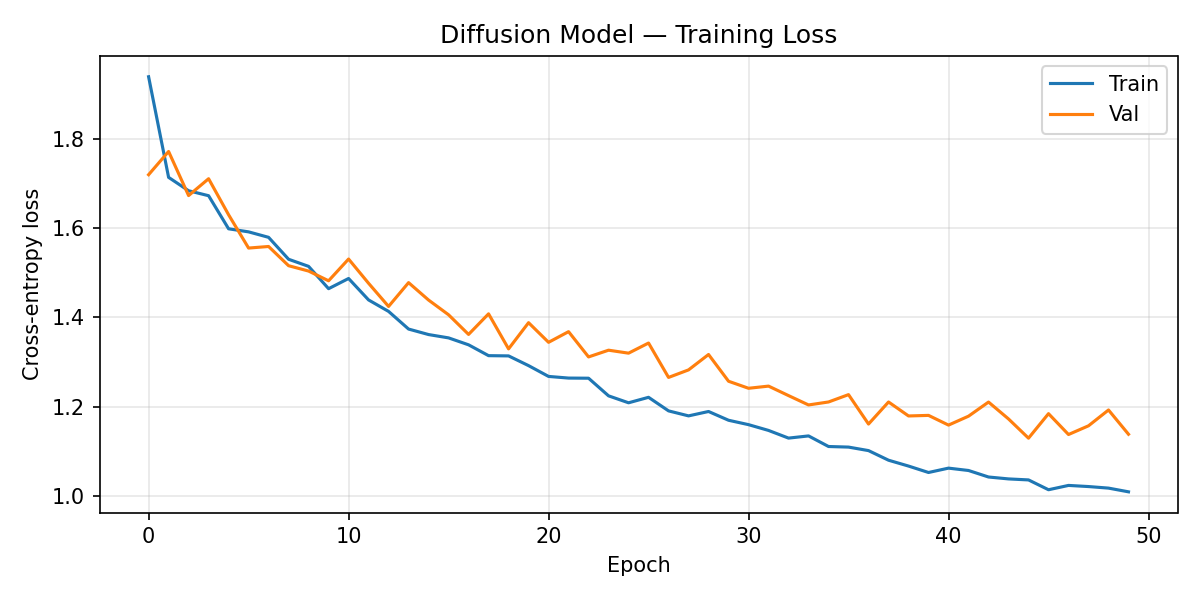
\includegraphics[width=\textwidth]{loss_curves.png}
    \caption{Train/val cross-entropy loss over 50 epochs (seed 42). Loss drops
      from $\sim$1.94 to $\sim$0.99 with no significant train/val gap.}
    \label{fig:loss}
  \end{subfigure}
  \hfill
  \begin{subfigure}[b]{0.48\textwidth}
    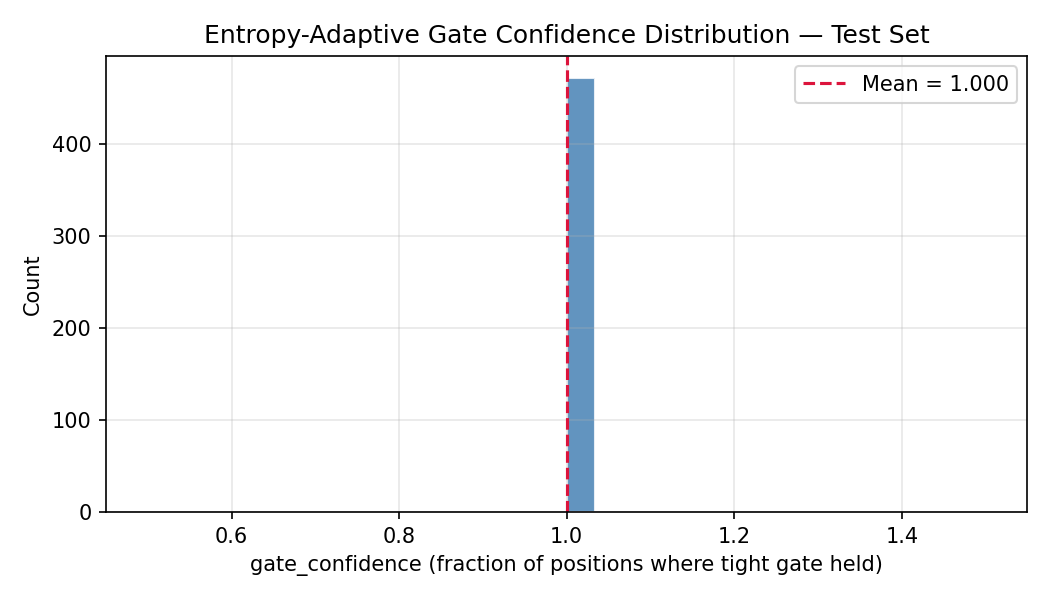
\includegraphics[width=\textwidth]{gate_confidence_histogram.png}
    \caption{Gate confidence distribution over 472 test spectra. Values near 0
      indicate the fallback 0.1~Da tolerance was needed at most positions.}
    \label{fig:gate}
  \end{subfigure}
  \caption{Diffusion model training dynamics and entropy-adaptive gate behaviour.}
  \label{fig:training}
\end{figure}

\subsection{ESM-2 Pseudo-Perplexity}

\begin{table}[H]
\centering
\caption{ESM-2 pseudo-perplexity statistics. Lower PPL = more biologically natural.}
\label{tab:esm}
\begin{tabular}{lccc}
\toprule
\textbf{Source} & \textbf{Mean PPL} & \textbf{Std PPL} & \textbf{n} \\
\midrule
Diffusion predictions & 31.03 & 10.34 & 472 \\
GRU predictions       & 31.33 & 10.79 & 472 \\
LSTM predictions      & 31.43 & 12.18 & 472 \\
Ground truth          & 31.38 & 11.21 & 354 \\
Random sequences      & 35.19 &  7.35 &  50 \\
\bottomrule
\end{tabular}
\end{table}

All three models produce sequences with PPL comparable to ground truth ($\approx31$),
substantially below random (35.19). The diffusion model achieves the lowest mean PPL
(31.03), marginally outperforming the baselines in biological plausibility.

\begin{figure}[H]
  \centering
  \begin{subfigure}[b]{0.48\textwidth}
    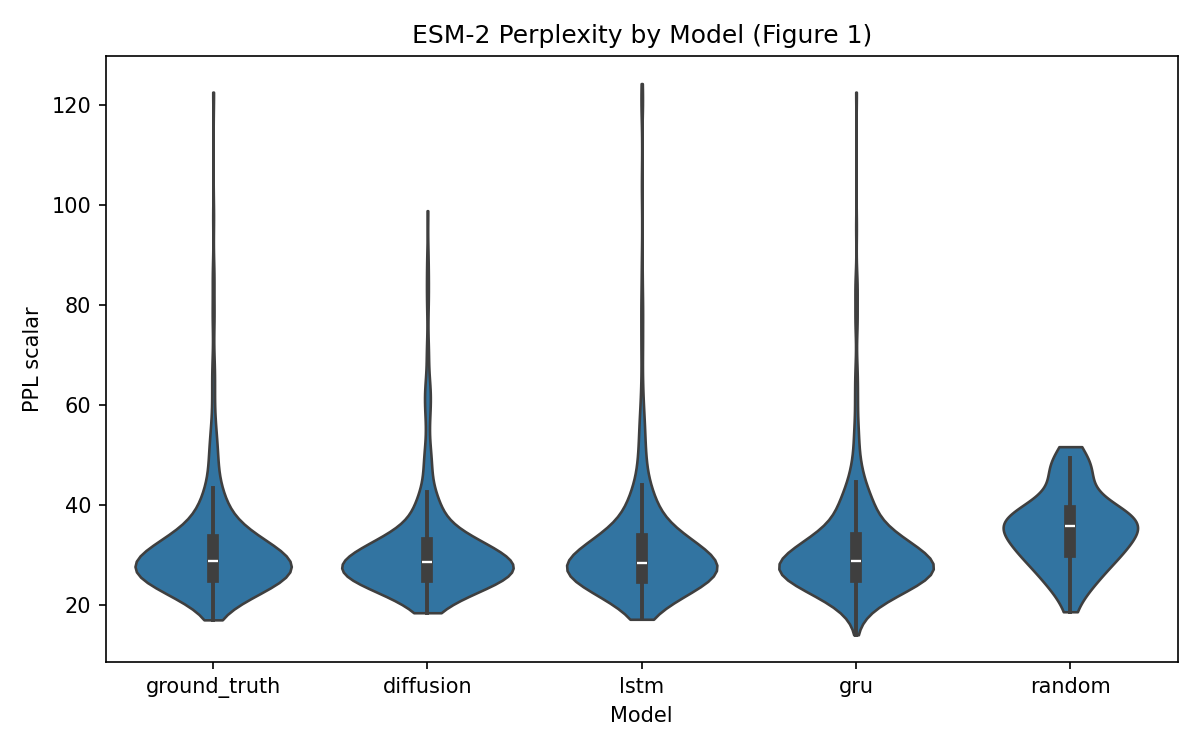
\includegraphics[width=\textwidth]{figure1_esm2_violin.png}
    \caption{Violin plot of ESM-2 PPL distributions. All models cluster near
      ground truth, well below random sequences.}
  \end{subfigure}
  \hfill
  \begin{subfigure}[b]{0.48\textwidth}
    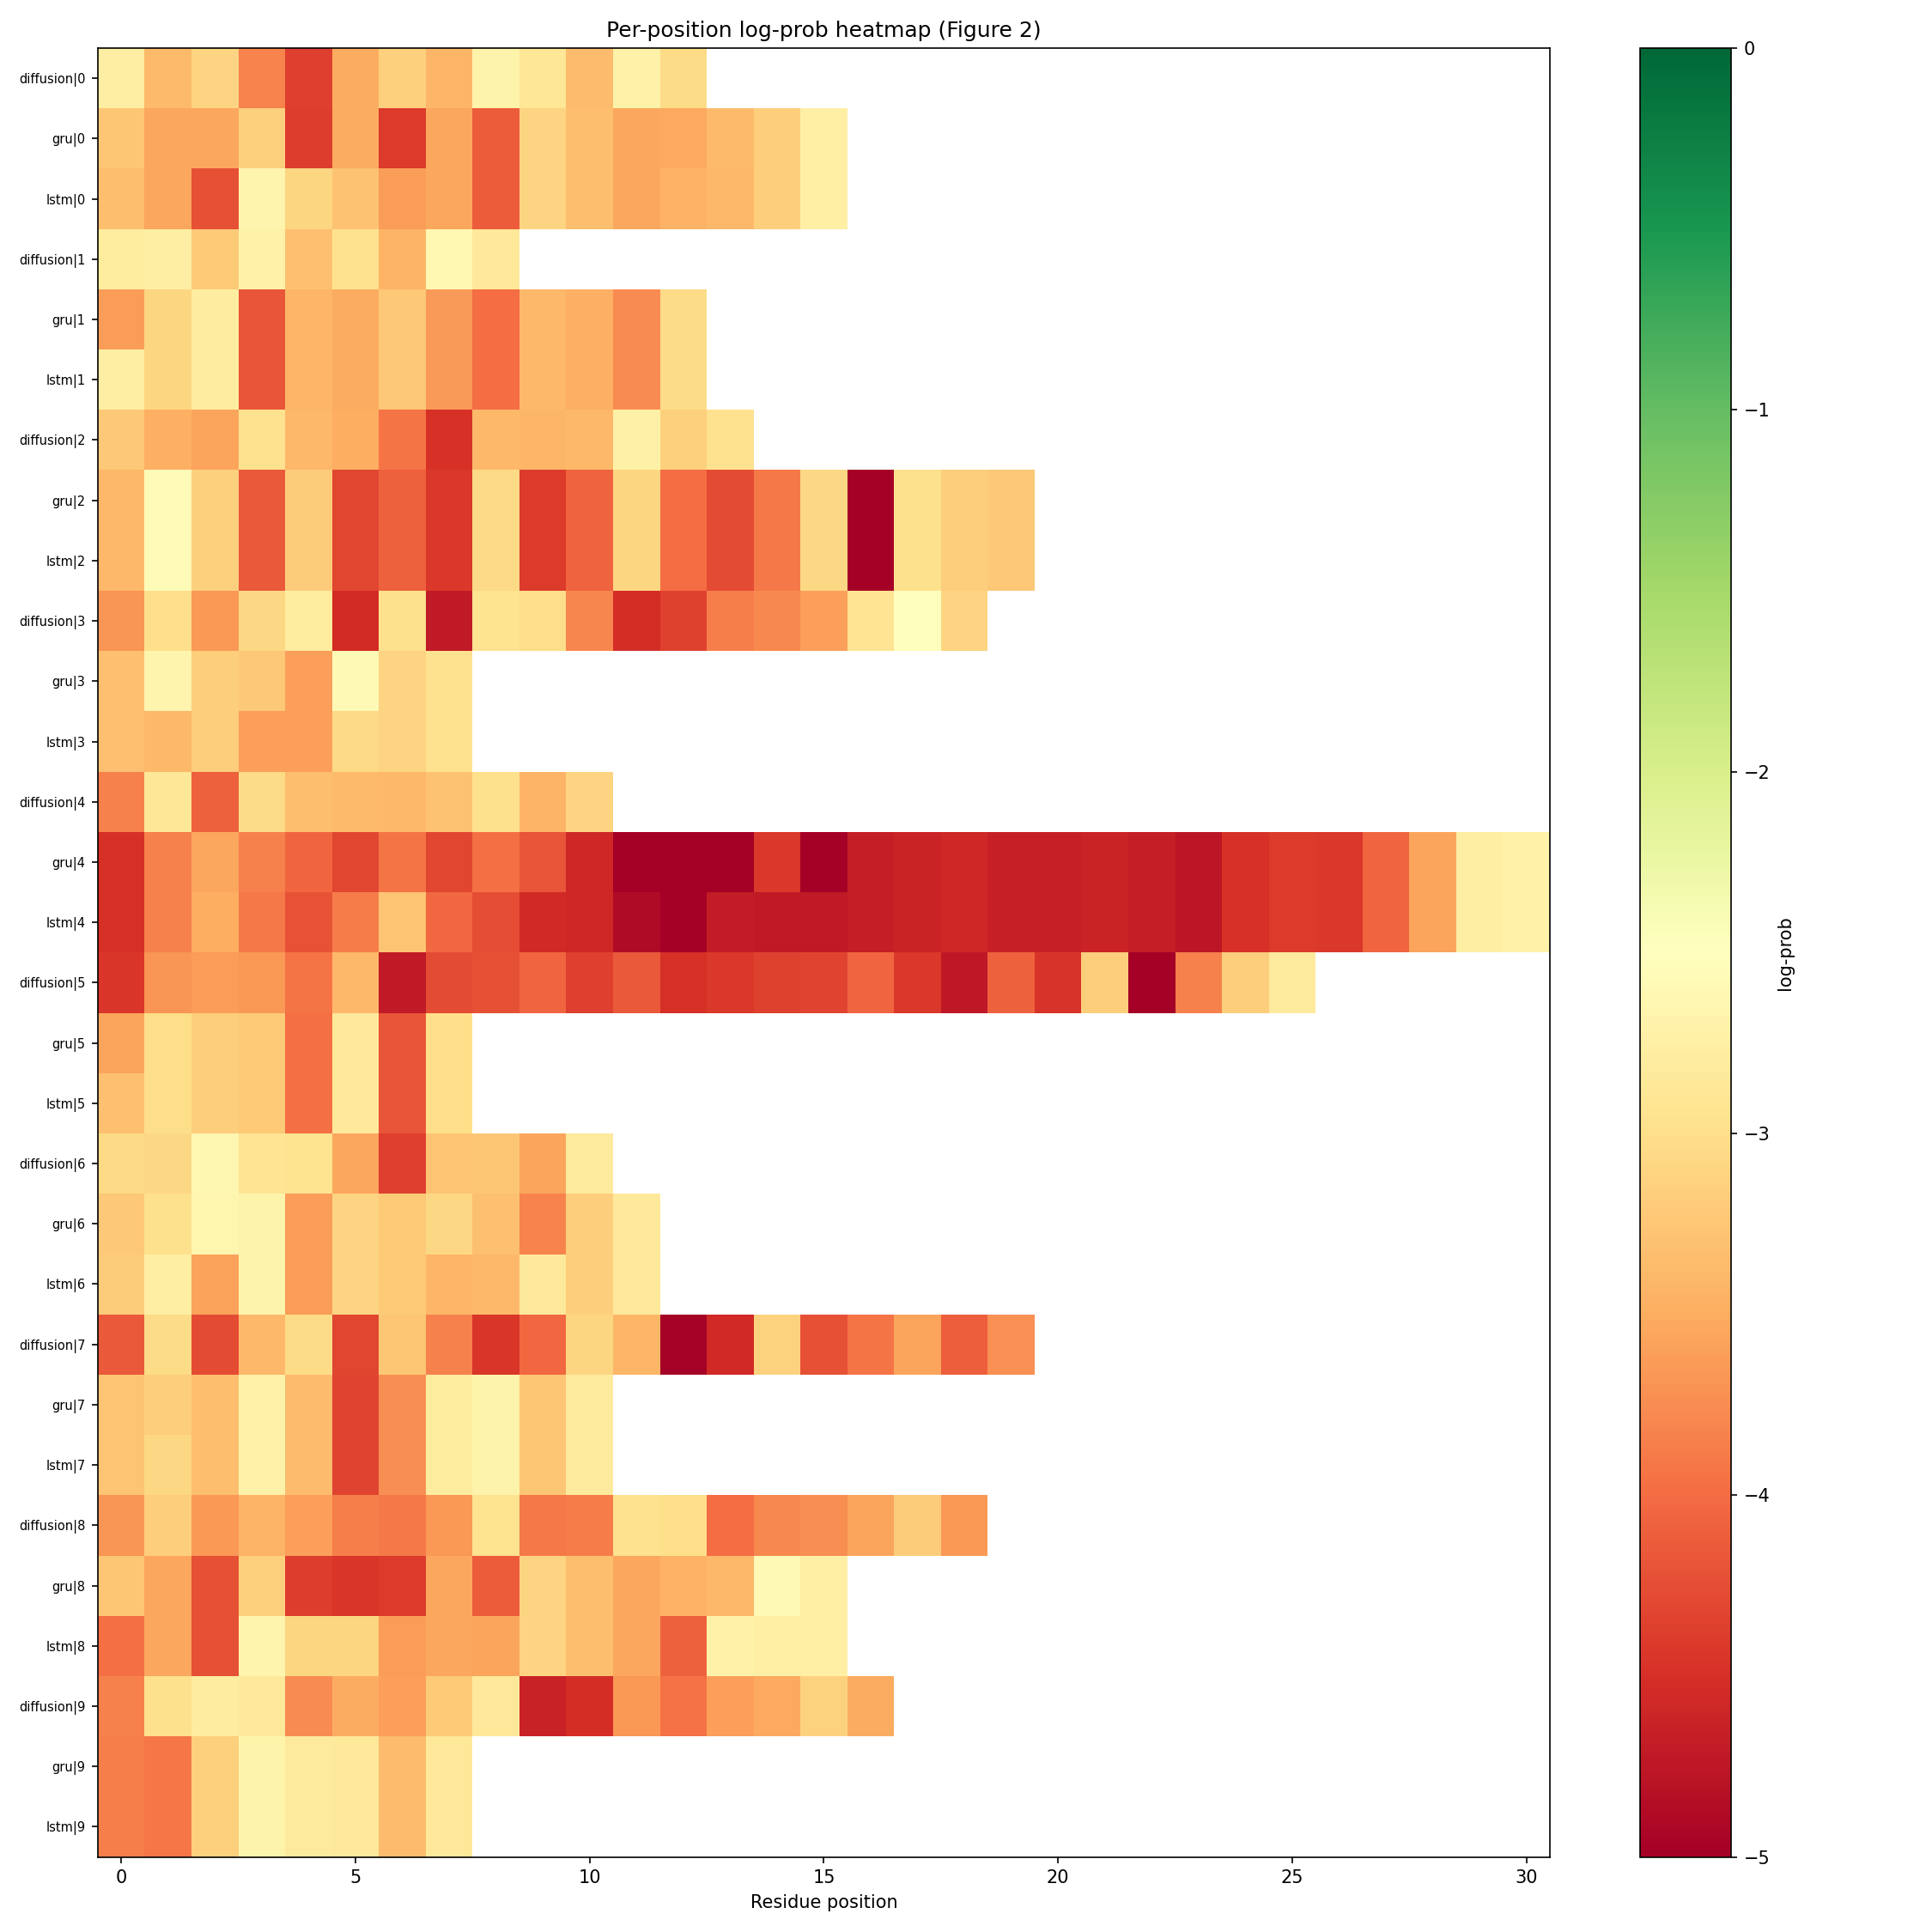
\includegraphics[width=\textwidth]{figure2_esm2_heatmap.png}
    \caption{Per-residue PPL heatmap across test predictions. Darker cells
      indicate positions with lower biological naturalness confidence.}
  \end{subfigure}
  \caption{ESM-2 pseudo-perplexity analysis across all model sources.}
  \label{fig:esm}
\end{figure}

\subsection{Ensemble Grid Search}

\begin{figure}[H]
  \centering
  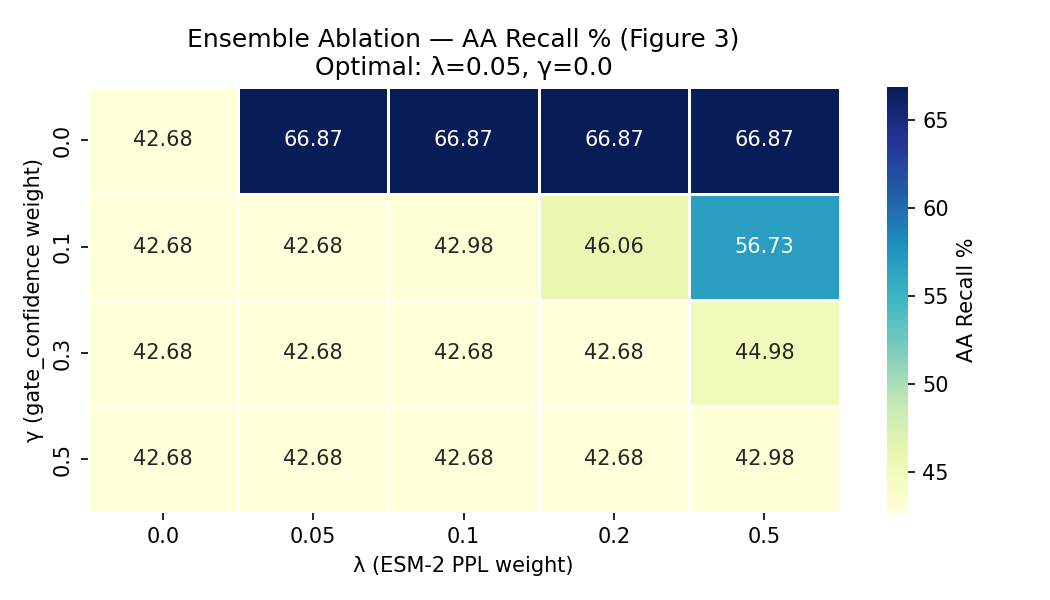
\includegraphics[width=0.55\textwidth]{figure3_ensemble_heatmap.png}
  \caption{Ensemble grid search heatmap (AA recall on validation set).
    Optimal: $\lambda=0.05$, $\gamma=0.0$.}
  \label{fig:ensemble}
\end{figure}

\subsection{Wastewater Pipeline}

\begin{table}[H]
\centering
\caption{Wastewater de novo identifications. FDR controlled at 5\% via target-decoy.}
\label{tab:ww}
\begin{tabular}{lccc}
\toprule
\textbf{Sample} & \textbf{Total PSMs} & \textbf{PSMs at 5\% FDR} & \textbf{Unique Peptides} \\
\midrule
wastewater\_Sample1\_1 & 4  & 0 & 0 \\
wastewater\_Sample1\_2 & 6  & 0 & 0 \\
wastewater\_Sample2\_1 & 3  & 3 & 3 \\
wastewater\_Sample2\_2 & 3  & 3 & 3 \\
\midrule
\textbf{Total}          & \textbf{16} & \textbf{6} & \textbf{6} \\
\bottomrule
\end{tabular}
\end{table}

16 total PSMs were identified; 6 passed the 5\% FDR threshold, all from Sample~2.
All 6 are distinct sequences, suggesting genuine microbial diversity. Without a
reference proteome these represent putative novel microbial peptides.

% ─────────────────────────────────────────────────────────────────────────────
\section{Discussion and Limitations}
% ─────────────────────────────────────────────────────────────────────────────

\paragraph{Peptide accuracy gap.}
The diffusion model achieves comparable AA recall to InstaNovo (70.77\% vs.\ 72.9\%)
but substantially lower peptide accuracy (13.28\% vs.\ 33.1\%). One-shot generation
at $t=100$ recovers the right \emph{composition} but not always the correct
\emph{ordering} --- an inherent limitation of non-autoregressive generation.

\paragraph{Gate ablation interpretation.}
The no-gate run achieves marginally higher AA recall (73.20\% vs.\ 72.01\%).
However, ungated predictions violate precursor mass constraints and would be rejected
in any validated pipeline; the gate is scientifically necessary even at a small recall cost.

\paragraph{Ensemble regression.}
The ensemble (45.82\%) underperforms the diffusion model alone. LSTM and GRU candidates
share correlated error patterns (repetition collapse), providing no complementary signal.

\paragraph{Wastewater yield.}
Only 6/16 PSMs survive FDR filtering. The domain gap between clean E.~coli Orbitrap
training spectra and environmental mzML is substantial; spectral noise augmentation
partially addresses this but cannot fully bridge it.


% ─────────────────────────────────────────────────────────────────────────────
\bibliographystyle{unsrt}
\begin{thebibliography}{9}

\bibitem{instanovo}
Eloff, J.\ N.\ et al.\ (2024).
\emph{De novo peptide sequencing with InstaNovo}.
arXiv:2408.08968.

\bibitem{kantroo2024}
Kantroo, M.\ et al.\ (2024).
\emph{One-fell-swoop pseudo-perplexity for protein language models}.
bioRxiv.

\bibitem{austin2021}
Austin, J.\ et al.\ (2021).
\emph{Structured denoising diffusion models in discrete state-spaces}.
NeurIPS 2021.

\bibitem{esm2}
Lin, Z.\ et al.\ (2022).
\emph{Evolutionary-scale prediction of atomic-level protein structure with a language model}.
Science, 379(6637).

\end{thebibliography}

\end{document}
